\documentclass[10pt]{beamer}
\usetheme{pohan}
\usepackage{lipsum}
\usepackage{tabularx}
\usepackage{xcolor}
\usepackage{fancybox, graphicx}
\usepackage{animate}



\renewcommand{\arraystretch}{2}
\renewcommand\tabularxcolumn[1]{m{#1}}
\title{3/18 Paper Intro}
\subtitle{ + Paper Report Questions}
\author{Pohan Chi}
\date{\today}


\begin{document}

\maketitle

\maketoc

\section{Mogrify LSTM}

\begin{frame}{Title}

    \begin{figure}
        \centering 
        \shadowbox{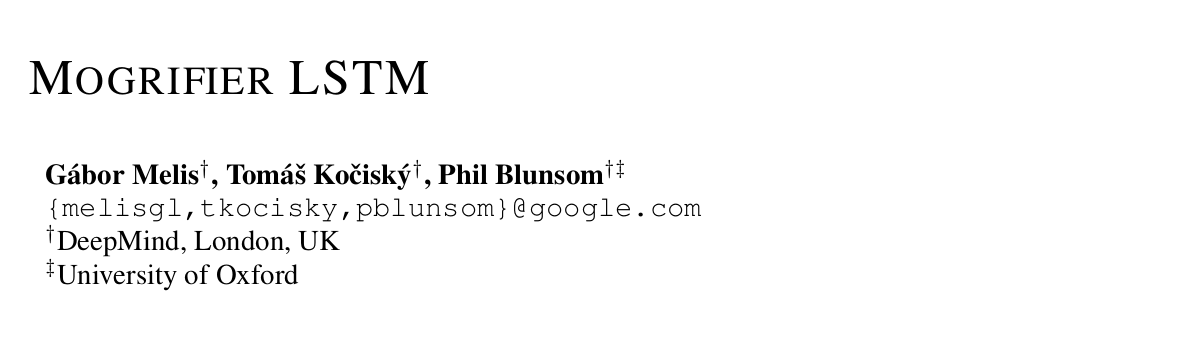
\includegraphics[width=0.95\textwidth]{img/mogrifier}}
    \end{figure}

\end{frame}

\begin{frame}{Mogrify LSTM - Motivation}
    \begin{enumerate}
        \item Improve Generalization ability of Language Model
        \item Amplify salient and attenuate nuisance features in the input embeddings
        \item Context-free representation is a bottleneck in LM
        \item conditioning the input embedding on the recurrent state will improve performance. 
    \end{enumerate}
\end{frame}

\begin{frame}{Mogrify LSTM - Model}

    \begin{figure}
        \begin{center}
            \shadowbox{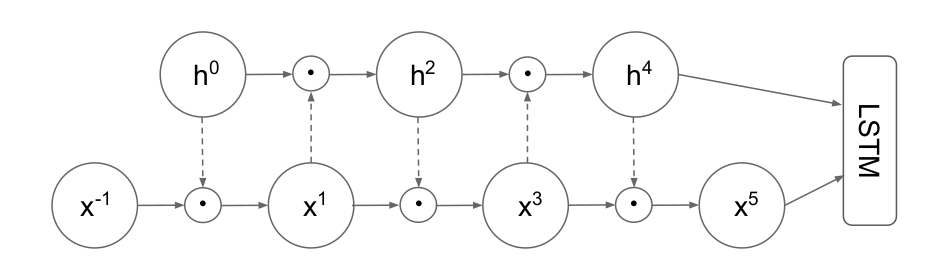
\includegraphics[width=0.95\textwidth]{img/mogrifier-model}}
        \end{center}
    \end{figure}

\end{frame}

\begin{frame}{Mogrify LSTM - partial Experiments}

\end{frame}

\begin{frame}{Mogrify LSTM - Insight}

\end{frame}

\section{SBERT-WK}

\begin{frame}{Title}
    
\end{frame}

\begin{frame}{SBERT-WK - Motivation}
    

\end{frame}

\begin{frame}{SBERT-WK - Model}

    \begin{figure}
        \begin{center}
            \shadowbox{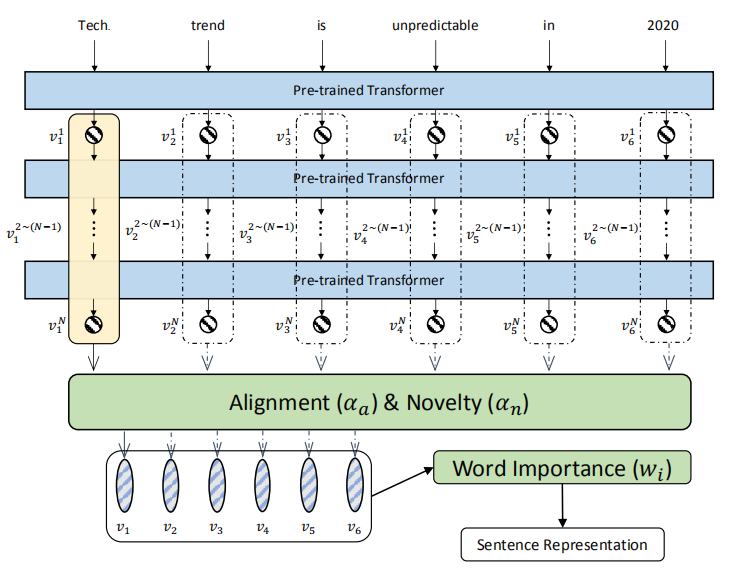
\includegraphics[width=0.82\textwidth]{img/SBERT-WK-model}}
        \end{center}
    \end{figure}

\end{frame}

\begin{frame}{SBERT-WK - partial Experiments}

\end{frame}

\begin{frame}{SBERT-WK - Insight}

\end{frame}

\section{Generalization through Memorization: Nearest Neighbor Language Models}

\begin{frame}{Title}
    
\end{frame}

\begin{frame}{knn-LMs - Motivation}

\end{frame}

\begin{frame}{knn-LMs - Model}

\end{frame}

\begin{frame}{knn-LMs - parital Experiments}

\end{frame}

\begin{frame}{knn-LMs - Insight}

\end{frame}

\section{Differentiable Reasoning over a Virtual Knowledge Base}

\begin{frame}{Title}
    
\end{frame}

\begin{frame}{Recap}
    
\end{frame}

\begin{frame}{Question 1}

\end{frame}

\begin{frame}{Question 2}

\end{frame}

\begin{frame}{Question 3}

\end{frame}

\begin{frame}{Question 4}

\end{frame}


\end{document}
